\chapter{Modeling Risk Correlation}

In credit derivative valuation and credit risk management, one of the most important issues is the estimate of default probabilities and their correlations. Two are the possible ways to address this task: using historical default data or mathematical models.

Historical default data has played an important role in the estimate of default probabilities in the past. However, because credit events are rare, there is very limited data available. Moreover, historical data only reflects the past default patterns and it may not be a proper indicator of the future. This makes such technique difficult and inexact. To use this same data to estimate default correlations is even more difficult and inexact.

The market trend now is towards the use of mathematical models that don't rely on historical default data. In Chapter~\ref{sec:credit-default-swaps} we have seen how it is possible to derive default probabilities from market data, here we will see how copulas can be used to model their correlations to evaluate credit derivatives. 

\section{Default Correlation}
\label{sec:default_correlation}

Correlation is a precise mathematical concept that has only meaning in reference to random variables. If $X$ and $Y$ are random variables, the \emph{correlation coefficient}, $\rho$, between $X$ and $Y$ is defined as
\begin{equation}
\rho = \cfrac{\mathbb{E}[(X-\mu_Y)(Y-\mu_Y)]}{\sigma_X \sigma_Y}
\label{eq:correlation_coefficient}
\end{equation}
where $\mu$ and $\sigma$ denote the corresponding mean and standard deviation, and $\mathbb{E}$ the expected value.

%Statements such as "company $A$ and company $B$ are correlated" are meaningless unless you refer to a quantifiable variable associated with the two companies (e.g. stock price, revenue growth or credit default spread).
Stating that the default behavior of companies $A$ and $B$ is correlated does not carry a lot of meaning unless one specifies a random variable that captures what \emph{default behavior} means.

The challenge to do a good Monte Carlo simulation to model asset defaults relies on the ability to generate realistic scenarios. That is, being able to be loyal to the average default probability of the pool and to the assets’ default correlation $\rho$. Note that if we are dealing with two assets, the default correlation is captured by one number. In the case of $N>2$ assets, $\rho$ is a symmetric matrix (sometimes also indicated by $\Sigma$).

\begin{equation*}
\Sigma = \begin{bmatrix}
\sigma^2 (X_0) & \cov(X_0, X_1) & \cov(X_0, X_2)\\
 \cov(X_1, X_0) & \sigma^2 (X_1) & \cov(X_1, X_2)\\
 \cov(X_2, X_0) & \cov(X_2, X_1) & \sigma^2 (X_2)\\
\end{bmatrix}
\end{equation*}
 
Diagonal terms report the variance of each random variable, while the non-diagonal terms represent the correlation between each pair of variables. The matrix is symmetric since the correlation between $X_i$ and $X_j$ is the same as between $X_j$ and $X_i$.

\section{Distribution Transformation}
\label{distribution-transformation}

Distribution transformation is a very useful tool which will be extensively used with the copula. This technique allows to transform every random variable distribution into uniform and vice versa and is called \emph{inverse transform} (or \emph{probability integral transform}).
It involves computing the cumulative distribution function $F_{X}$ (or its inverse) which maps a number to a probability between 0 and 1. 

\begin{attention}
\subsubsection{Demonstration}
Let's start with a random variable $X$ and let $F_X$ be its cumulative distribution function ($F(x) = P(X \leq x)$).
We would like to find a transformation $T:[0,1]\rightarrow\mathbb{R}$ such that $T(U)=X$, where $U$ is the uniform distribution in $[0,1]$. 
\begin{equation*}
F_X(x)= P(X\leq x)=P(T(U)\leq x)= P(U\leq T^{-1}(x))=T^{-1}(x),{\text{ for }}x\in \mathbb {R}
\end{equation*}
where the last step used that $P(U\leq y)=y$ when $U$ is uniform on $(0,1)$.

So we got $F_{X}$ to be the inverse function of $T$, or, equivalently $T(u)=F_{X}^{-1}(u)$, $u\in [0,1]$, hence $T$ is the \textbf{quantile function}.
\end{attention}

To transform a generic random variable to uniform (and vice versa) we can use
\begin{equation}
x = F_{X}^{-1}(u)\quad\mathrm{and}\quad u = F_X(x)	
\end{equation} 
\noindent Figure~\ref{fig:inverse_transform} shows graphically how the inverse transform works.

\begin{figure}[htb]
\centering
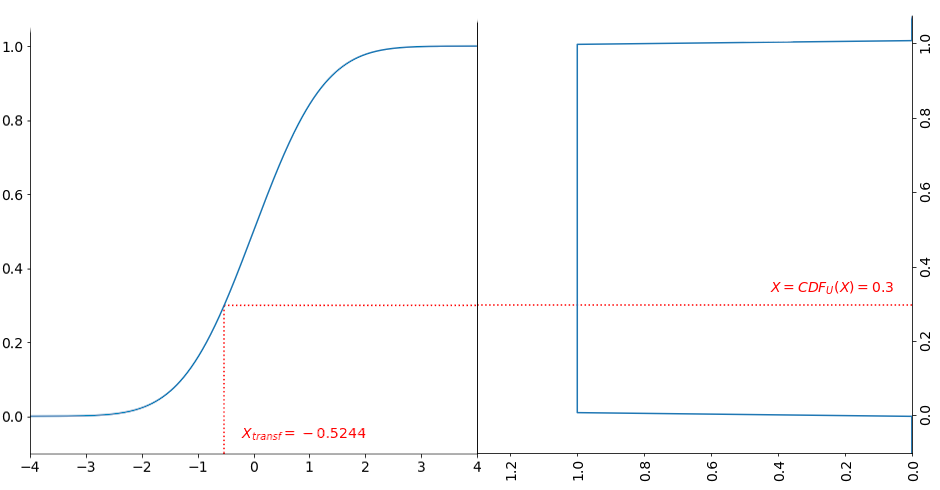
\includegraphics[width=0.9\textwidth]{figures/inverse_transform}
\caption{Inverse transform example. Going from right to left a sample $x$ in $[0,1]$ interval is chosen, this corresponds also to CDF$_{\text{U}}(x)$. This value is selected on the CDF of the other distribution $f$ and it is finally transformed into a sample from $f$ using the quantile function.}
\label{fig:inverse_transform}
\end{figure}

Imagine we want to transform a uniform distribution into Gaussian. The transformation takes uniform samples $u$ between 0 and 1, interpreted as a probabilities, and then returns $F_{\text{normal}}^{-1}(u)$. The following code shows how this can be done in \texttt{python}. 

\pythoncode{code/modelling_risk_1.py}

We start by generating a sample from the uniform distribution using \texttt{scipy.stats.uniform}, line 3. 
In the left plot of Fig.~\ref{fig:a_to_b_to_a} the resulting distribution is shown.
Next we want to transform the sample so that it becomes normally distributed. The transformation to use is the quantile function of the normal distribution, or $(\tt{ppf(x))}$. Remember that all the methods of \texttt{scipy.stats} applied to \texttt{numpy.array} works on each item of the array without the need to make explicit for-loops.
In the mid plot of Fig.~\ref{fig:a_to_b_to_a} the Gaussian obtained with the code below is shown

\begin{figure}[htbp]
	\centering
	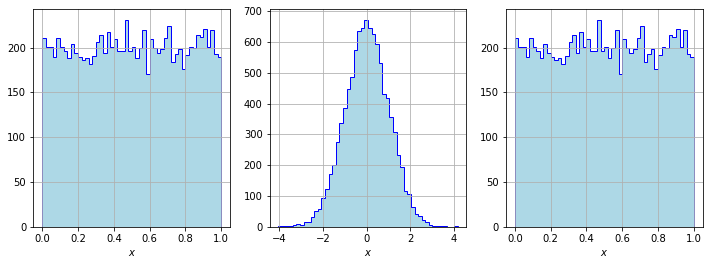
\includegraphics[width=0.8\textwidth]{figures/a_to_b_to_a}
	\caption{Example of transformation, it starts with a uniform distribution, goes into a Gaussian and back to the initial uniform.}
	\label{fig:a_to_b_to_a}
\end{figure}

If we plot the two distribution together we can get a sense of what is going on using the inverse CDF transformation. Indeed it stretches the outer regions of the uniform to yield a normal distribution. This is shown in Fig.~\ref{fig:uniform_to_gauss}. 
    
\begin{figure}[htbp]
\centering
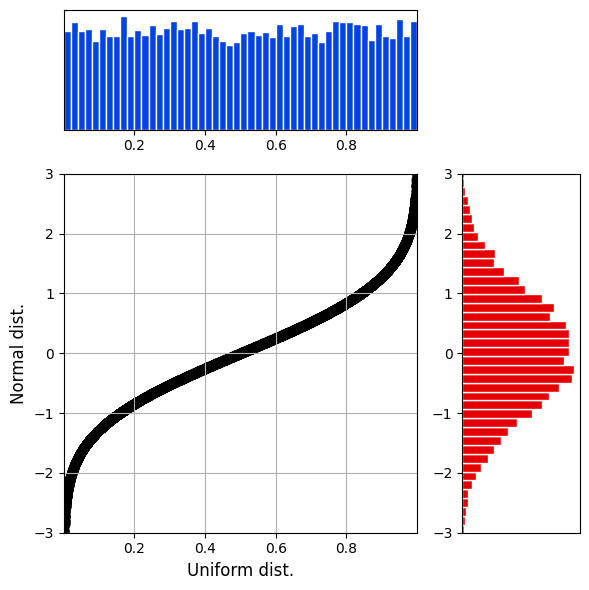
\includegraphics[width=0.6\textwidth]{figures/uniform_to_gauss}
\caption{2D plot showing the transformation that maps our initial uniform distribution to the resulting Gaussian.}
\label{fig:uniform_to_gauss}
\end{figure}
    
Clearly to do the opposite transformation, that is from an arbitrary distribution to uniform, we can just apply the inverse of the inverse CDF, that is the CDF itself, line 5.
In such a way we can go from distribution A to B passing through the uniform rather quickly as shown in three plots of Fig.~\ref{fig:a_to_b_to_a}.

Notice that this technique can be used for any arbitrary (univariate) probability distribution so you can test it with different samples. 

\section{Copula}
\label{copula}

A \emph{copula} $\mathcal{C}(F_1, F_2, \ldots, F_n, \rho)$ allows the joining of multiple univariate distributions to a single multivariate distribution. Copulas are used to describe the dependencies between random variables and have been widely used in quantitative finance to model risk. 

Its exact definition from probability theory is the following: a multivariate, i.e. multidimensional, cumulative distribution function whose \emph{marginal} probability distributions, i.e. the probability distribution of each dimension, are uniform ($F_i = U_i =\mathrm{uniform}(0,1)$), $\rho$ represents the correlation between each variable.

A key part of copulas is the \emph{Sklar’s theorem}. It states that any multivariate joint distribution can be written in terms of the marginal distributions and a copula which describes the dependence structure between the variables. This property makes them very popular since allow to easily model the distribution of correlated random variables by representing marginals and correlation separately: essentially allow to split a complicated problem into simpler components.

\begin{attention}
Mathematically, the theorem can be stated as follows: suppose we have only two random variables, $X$ and $Y$. If $F(x,y)$ is a joint distribution function with continuous marginals $f_x(x)=u$ and $f_y(y)=v$, then the joint distribution $F(x,y)$ can be written in terms of a unique function $\mathcal{C}(u,v)$:
\begin{equation}
F(x,y)=\mathcal{C}(u,v)
\end{equation}
\noindent
where $\mathcal{C}(u,v)$ is the copula of $F(x,y)$.
The copula function describes how the multivariate function $F(x,y)$ is derived from or coupled with the marginal distribution functions $f_x(x)$ and $f_y(y)$.
\end{attention}

Despite the probably obscure and daunting definition given above the concept of copula is quite simple so it will be clarified with a practical example.

\section{Working with Correlated Distributions}
\label{sec:generate-correlated-distributions}

\subsection{Correlated Asset Returns}
\label{sec:correlated_stock_returns}

In this example we are going to consider the closing prices of two assets like BMW and Siemens in the period between 2010 and 2022 (the series can be found in \href{https://github.com/matteosan1/finance_course/raw/master/input_files/bmw_siemens.csv}{bmw\_siemens.csv}).

Since the two companies belongs to the same sector and to the same market it is plausible to assume that their returns are correlated, and in particular we would like to estimate the probability that both of them are negative.

From the historical series of the two assets we can determine the distributions of the individual returns irrespective of the other one, i.e. the marginals, but we don't know how we could model the correlated probability distribution, \emph{joint distribution}, with which we should work to answer our question. 

Here is where copula comes in hand, since it bridges the marginal distributions (which by definition have no correlation) into a joint probability distribution. 

\pythoncode{code/modelling_risk_2.py}

In the code we first load the historical series and check the correlation between the two assets (lines 5-6).
\begin{ioutput}
          BMW.DE    SIE.DE
BMW.DE  1.000000  0.664654
SIE.DE  0.664654  1.000000
\end{ioutput}
Indeed the returns are correlated by about 66\% as shown in Figure~\ref{fig:bmw_sie_returns}.

\begin{figure}[htbp]
\centering
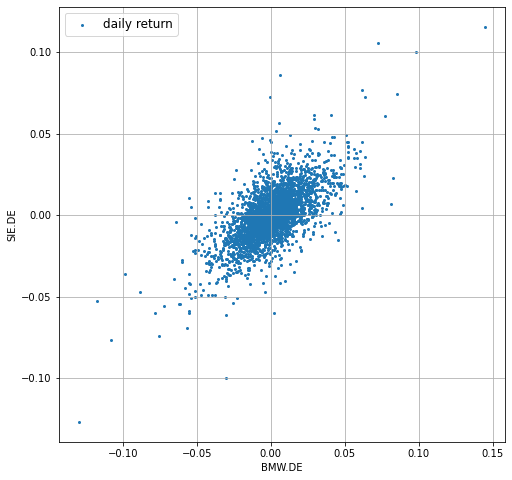
\includegraphics[width=0.6\textwidth]{figures/bmw_sie_daily_returns}
\caption{Distribution of the daily returns of BMW and Siemens stock price from 2010 to 2022.}
\label{fig:bmw_sie_returns}
\end{figure}

By fitting the return histograms, e.g. using t-student~\cite{bib:t_student} functions, we can determine the parametric form of the marginal distributions. The resulting fits are shown in Fig.~\ref{fig:bmw_sie_fit}.

\begin{figure}[htbp]
\centering
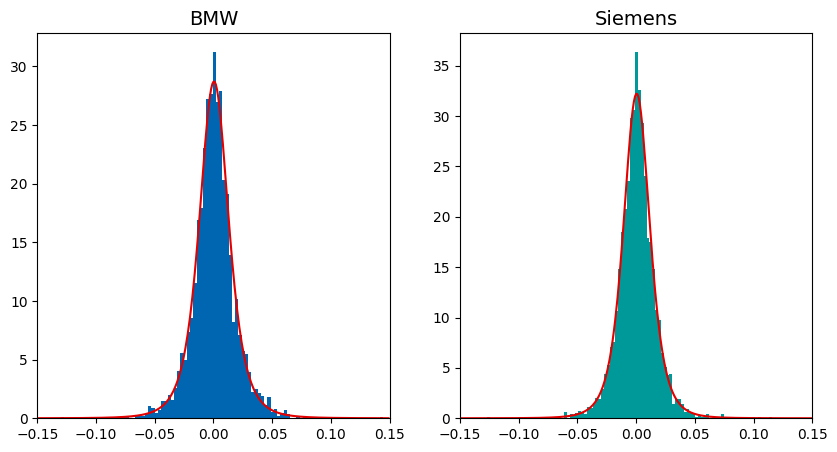
\includegraphics[width=0.75\textwidth]{figures/bmw_siemens_fit}
\caption{Fit of the daily return distributions for BMW (left) and Siemens (right). The assumed functional form is a t-student.}
\label{fig:bmw_sie_fit}
\end{figure}

\begin{finmarkets}
\label{sec:how_to_fit}
Histogram fitting is the art of choosing a probability model for the unknown population, and calibrating that model (setting the best value for the model parameters) using a representative sample from the population.

In \texttt{python} this can be done quite easily since each \texttt{scipy.stats} distribution has a convenient method \texttt{fit} which performs the calibration and return an array with the best estimate of the parameter values.
\end{finmarkets}

To model the joint probability distribution we first have to simulate a sample from a multivariate distribution with the specific correlation structure, lines 15-16. To keep thing simple we are going to assume a Gaussian correlation, this is not mandatory though, since we could have modeled it with different distribution either.
It is important to understand that correlation doesn't affect the distribution of each component, but it rather changes how given a sample the second is determined.

We then transform the sample so that the marginals are uniform with the technique outlined above (obtaining the copula function). This is done with the \texttt{cdf} transformation in line 18 and the result is shown in Fig.~\ref{fig:copula}. Plots like this are how copulas are usually visualized. Since we have used a multivariate standard normal to model the correlation this is an example of \textbf{Gaussian Copula}.

\begin{figure}[htbp]
	\centering
	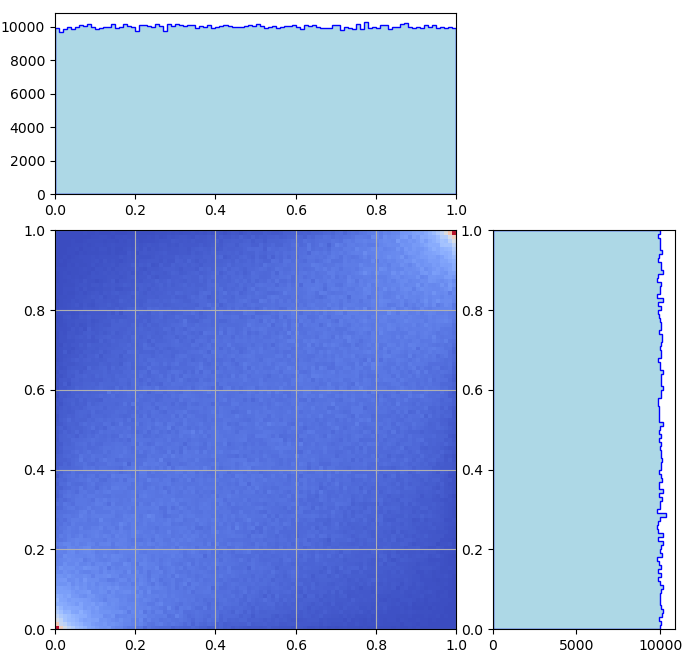
\includegraphics[width=0.45\textwidth]{figures/copula_2d}
	\quad
	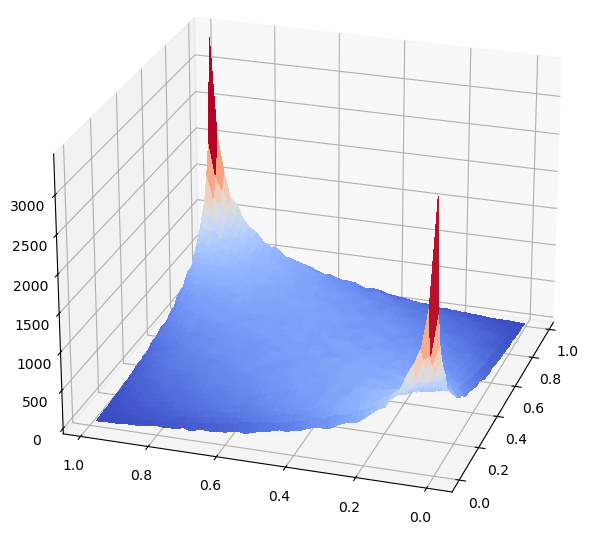
\includegraphics[width=0.5\textwidth]{figures/copula_3d}
	\caption{Graphical representations of the copula, 2D on the left, 3D on the right.}
	\label{fig:copula}
\end{figure}

At this point we can just transform the uniform marginals to the appropriate distributions (t-students in our case) to have the desired correlated distributions. This is done using the corresponding \texttt{ppf} transformations in lines 20-21.

To see that it is actually working as expected we have compared the two joint distributions (with and without correlation) and computed the probability to have both stocks going down at the same time in the two cases.
Note that to compute the probability, ignoring the correlation between the returns, we have just sampled from the two marginals (lines 23-24) and counted how many times they both are negative.

\begin{ioutput}
Probability w/ correlation: 0.3537
Probability w/o correlation: 0.2377
\end{ioutput}

The comparison between the two multivariate distributions in Figure~\ref{fig:bmw_sie_with_corr} clearly shows the different populations in the area of interest (shaded in yellow).

\begin{figure}[htbp]
\centering
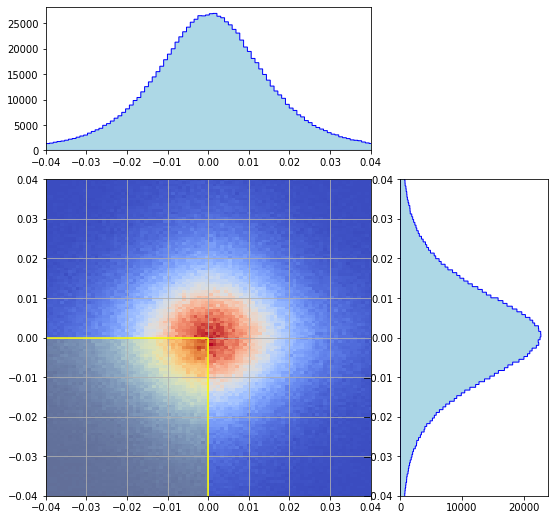
\includegraphics[width=0.45\textwidth]{figures/bmw_sie_uncorrelated}
\quad
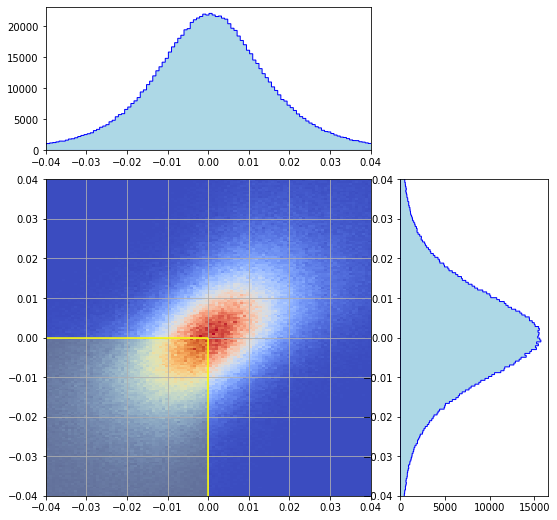
\includegraphics[width=0.45\textwidth]{figures/bmw_sie_correlated}
\caption{Marginalized t-student distributions with their joint when they are (right) and are not (left) correlated.}
\label{fig:bmw_sie_with_corr}
\end{figure}
    
Using the uniform distribution as a common base for our transformations we can easily introduce correlations and flexibly construct complex probability distributions. Everything discussed in this Section could be easily generalized to higher dimensions.

\begin{finmarkets}
It may be useful to create a \texttt{python} object to handle copulas. In \texttt{finmarkets} this class is \texttt{GaussianCopula} and has a method \texttt{sample} which generates a sample from the Gaussian copula with the proper correlation.
\end{finmarkets}

\pythoncodenon{code/modelling_risk_3.py}

\subsubsection{Remarks on Gaussian Copula}
Extreme, synchronized rises and falls in financial markets occur infrequently but they do occur. The problem with Gaussian models is that they did not assign a high enough likelihood of occurrence to the scenario in which many things go wrong (or right) at the same time the “perfect storm” scenario.

To make this statement a little bit more quantitative we can determine the probability of a $5\sigma$ event and then compare it with the actual distribution of such events in finance. Notice that if $P$ is the probability of an event, $1/P$ represents its occurrence frequency, e.g. $P=0.5$ means the events is going to happen once every 2 trials.

\begin{attention}
A $n\sigma$ event has a probability to happen equivalent to that of sampling a value bigger than $n$ from a normal distribution.
To compute the occurrence frequency (in years) of such an event consider the probability to get $n\sigma$ so it is 1 over $(
[365\cdot P(|x| \ge n\sigma)]$ (the 365 factor comes from the number of working days in a year).

\pythoncodebox{code/modelling_risk_4.py}
\begin{ioutput}
4778.843544161504
\end{ioutput}
\noindent
\end{attention}

From the above calculation we expect to have a $5\sigma$ movement of our stock once every about 4800 years, assuming a Gaussian distribution. Looking the the distributions of the returns in the last 12 years in Fig.~\ref{fig:5sigma_contour}, where the red line represents the $5\sigma$ contour it is apparent that there are about twelve of such events instead.

\begin{figure}[htbp]
\centering
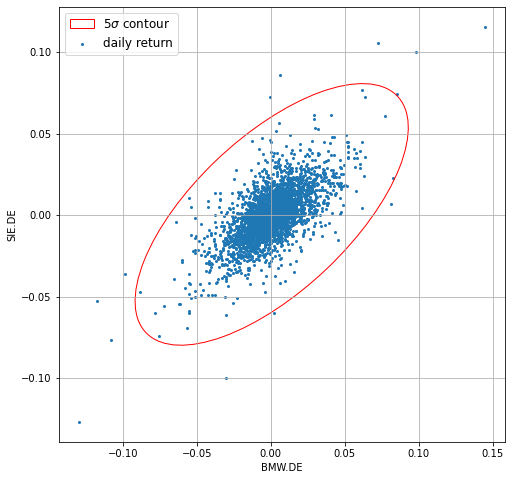
\includegraphics[width=0.5\textwidth]{figures/5_sigma_contour}
\caption{Distribution of the daily returns of BMW and Siemens stock price from 2010 to 2022, the red line represents the $5\sigma$ contour.}
\label{fig:5sigma_contour}
\end{figure}

When using a Gaussian copula, naturally assigns very little \emph{weight} to the tails. Hence it is often used the t-student copula which has fatter tails but preserves the same (bell shaped, non-skewed) characteristics of the Gaussian, see Section~\ref{sec:t-student_copula}. Indeed a $5\sigma$ movement under a t-student PDF is expected to happen once every 6 months. 

\subsection{Correlated Defaults}

Imagine a company with probability of defaulting within the next year equal to $\Pdef$.

To simulate the credit event by Monte Carlo it can be thrown a random number from a uniform distribution between 0 and 1  then:
\begin{itemize}
\item if it is lower or equal to $\Pdef$ then there has been default;
\item if it is higher no default happened.
\end{itemize}

\pythoncodenon{code/modelling_risk_5.py}

In such a way we have a "successful" experiment with the desired probability.

\begin{ioutput}
0.2058
\end{ioutput}

To generate samples from correlated distributions it is enough to determine the copula function as described in the previous Section. At the end of the computation each component of the sample is now converted to a set of random numbers drawn from the proper joint distribution.

Imagine three companies ($A$, $B$ and $C$) which have a cumulative probability of defaulting within the next two years of 10\%.
Let's compare the probability to have the three of them all defaulting within the next two years in two cases: independent and perfectly correlated default probabilities.

\pythoncodenon{code/modelling_risk_6.py}

In the first case (independent probabilities), the odds to get three defaults within two years is equivalent to the product of the single probabilities, hence $P_{\mathrm{uncorr}} = 10\% \cdot 10\% \cdot 10\% = 0.1 \%
$.

\begin{ioutput}
Uncorrelated defaults
3D copula distribution (first two samples only)
[[0.91972954 0.72719545 0.95619535]
 [0.7409053  0.81691954 0.5108085 ]]
Measured P_def: 0.00096
\end{ioutput}

If we repeat the same Monte Carlo experiment with perfectly correlated default probabilities we have (notice that the covariance matrix has non-diagonal 0.99999999 entries to avoid numerical errors, they should be 1)

In this case the result is close to 10\%, like we had only one single company defaulting. 
Indeed given the perfect correlation either there is no default or three "simultaneous" defaults with 10\% probability.

\begin{ioutput}
Correlated defaults
3D copula distribution (first two samples only)
[[0.94531087 0.94533677 0.94534905]
 [0.3477901  0.347964   0.3478019 ]]
Measured P_def: 0.10233
\end{ioutput}


%\subsubsection{Independent Defaults}\label{independent-defaults}
%
%If the default times of the number of companies are independent,
%default probabilities can be
%calculated through multiplication and integration of the single default
%probability curves without Monte Carlo simulation.
%
%As an example, consider the probability to have two defaults among four
%companies. Let \(\tau_i\) be the default time of name \(i\) and \(F_i(t)\)
%its distribution. Then the probability that name 1 defaults second in
%the basket before time \(t\) is:
%
%\begin{equation}
%\begin{split}
%&\mathbb{P}((\tau_2\lt\tau_1)\cap (\tau_1\lt t)\cap (\tau_1\lt\tau_3)\cap (\tau_1\lt\tau_4)) +\\
%&\mathbb{P}((\tau_3\lt\tau_1)\cap (\tau_1\lt t)\cap (\tau_1\lt\tau_2)\cap (\tau_1\lt\tau_4)) =\\
%&\int_0^t{F_2 (s)\cdot (1-F_3 (s)) \cdot (1-F_4 (s))~dF_1(s)} +  \int_0^t{F_3 (s)\cdot (1-F_2 (s)) \cdot (1-F_4 (s))~dF_1(s)}
%\end{split}
%\label{eq:indep_default}
%\end{equation}
%
%Suppose the default probabilities of three companies, $A$, $B$ and $C$ are
%given as in the following table (in each interval are linear):
%
%\begin{center}
%	\begin{tabular}{|c|c|c|c|}
%		\hline
%		time in years & A & B & C \\
%		\hline
%		\hline
%		0 & 0 & 0 & 0 \\
%		1 & 0.022032 & 0.0317 & 0.035 \\
%		2 & 0.046242 & 0.0655 & 0.075 \\
%		3 & 0.07266 & 0.1022 & 0.121 \\
%		4 & 0.101233 & 0.142 & 0.153 \\
%		5 & 0.131885 & 0.1752 & 0.205 \\
%		\hline
%	\end{tabular}
%\end{center}
%and suppose that the default events of the three companies are
%independent. The integral in Eq.~\ref{eq:indep_default} can be solved by substitution:
%
%\[ \int_{x_0}^{x_1}{(1-F_B(x))(1-F_C(x))dF_A(x)}\]
%
%Setting \(t=m_A x + q_A\) it becomes:
%
%\[ \int_{m_A x_0 + q_A}^{m_A x_1 + q_A}{(1-F_B(x(t)))(1-F_C(x(t)))dt}\qquad\Big(\textrm{with}~x(t) = \cfrac{t -q_A}{m_A}\Big) \]
%and similarly for company $B$ and $C$.
%
%To convert it into \texttt{python} we can use \texttt{scipy.integrate.quad} to
%perform the integral and \texttt{numpy.interp} to determine the
%intermediate default probabilities.	
%	First to default prob at time (1) for company A: 0.02131
%	First to default prob at time (2) for company A: 0.04301
%	First to default prob at time (3) for company A: 0.06460
%	First to default prob at time (4) for company A: 0.08573
%	First to default prob at time (5) for company A: 0.10606
%	First to default prob at time (1) for company B: 0.03080
%	First to default prob at time (2) for company B: 0.06160
%	...
%	\end{Verbatim}
%\end{tcolorbox}

\section{Cholesky Transformation to Correlate Variables}
In Section~\ref{sec:cholesky} it has been shown that a given matrix, $[\Sigma]$ can be factored uniquely into a product $[\Sigma]=[L]^T [L]$, where $[L]$ is a lower triangular matrix with positive diagonal entries. The matrix $[L]$ is the Cholesky (or "square root") matrix.

The Cholesky matrix can also be used to correlate random variables. Indeed if $[\Sigma]$ is the covariance matrix of a set of random variables , it transforms them such that their covariances are given by $[\Sigma]$. 

The intuition behind that relies on the following statement: from the transformation properties of the Gaussian distribution it is known that if $X\approx\mathcal{N}(\tau,\Lambda)$ then the transformation $Y=BX+b$ results in $Y$ distributed as $Y\approx\mathcal{N}(B\tau +b,B\Lambda B^{T})$.

Now immagine that $X$ is sampled from a standard $n$-dimensional normal distribution (i.e. $X\approx\mathcal{N}(0,\mathbb{1})$, where $\mathbb{1}$ is the $n\times n$ identity matrix, then $Y=BX+b$ is distributed as $Y\approx\mathcal{N}(b,BB^{T})$, which is just plugging in $\tau=0$ and $\Lambda=\mathbb{1}$ in the relation above.

If you now want $Y$ to be distributed as $Y\approx\mathcal{N}(\mu,\Sigma)$, then you need to choose some transformation matrix $A$, such that $AA^{T}=\Sigma$. A good choice for that is the Cholesky decomposition because it is explicitly structured to fulfill this condition and there are standard functions in lots of libraries which compute it for you.

As a practical example, suppose that $X$ is a vector of independent standard normal variables. The matrix $[L]$ can be used to create a new vector $Z$ such that the covariance of $Z$ equals $[\Sigma]$.

\pythoncodenon{code/modelling_risk_7.py}

\begin{ioutput}
[[1.73205081 0.        ]
 [0.57735027 0.81649658]]
\end{ioutput}

Figure~\ref{fig:cholesky_norm} shows the original uncorrelated variable $X$ (left), and the transformed variable $Z$ with correlation $[\Sigma]$ (right).

\begin{figure}[htbp]
\centering
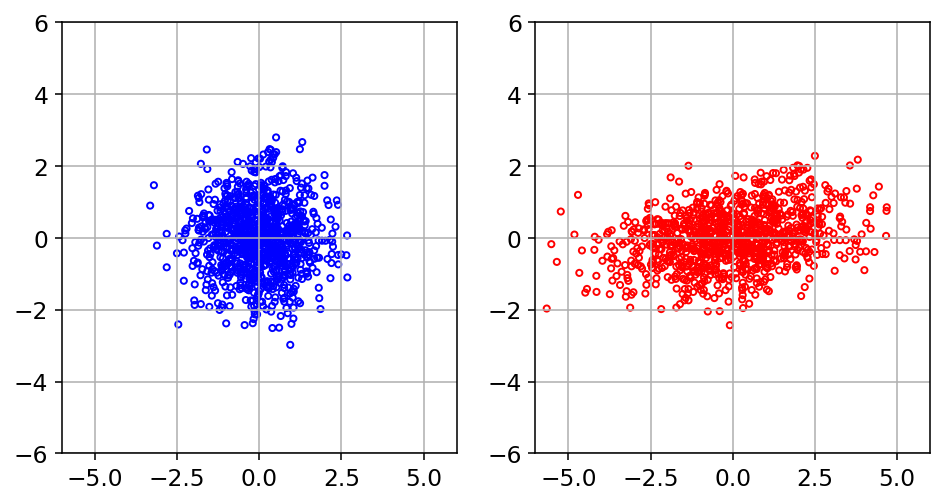
\includegraphics[width=0.7\textwidth]{figures/cholesky_norm}
\caption{The original uncorrelated variable $X$ (left), the transformed variable $Z$ (right).}
\label{fig:cholesky_norm}
\end{figure}

Clearly, if you start with correlated variables, you can apply the Cholesky inverse transformation to get uncorrelated variables.
If you take the $Z$ points generated above and apply $[L]^{-1}$, the original data is obtained again. Figure~\ref{fig:cholesky_inv} shows the resulting distribution.

\begin{ipythonnon}
orig_X = np.dot(Z, np.linalg.inv(L))
\end{ipythonnon}

\begin{figure}[htbp]
\centering
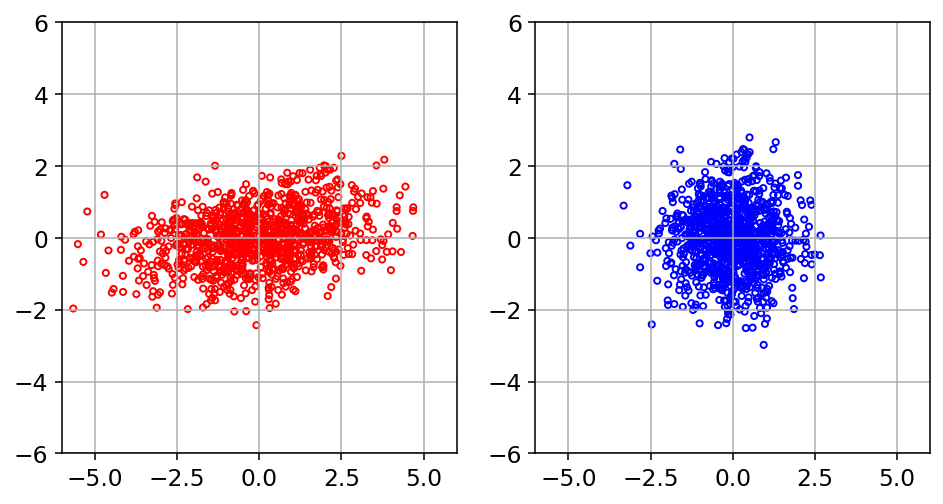
\includegraphics[width=0.7\textwidth]{figures/cholesky_inv}
\caption{The transformed variable $Z$ (left), and the original data obtained by the application of the inverse Cholesky transformation (right).}
\label{fig:cholesky_inv}
\end{figure}

\subsection{t-copula with $\chi^2$ Method}
\label{sec:t-student_copula}
The t-student copula allows a range of dependence structures depending
on the $\nu$ parameter (the number of degrees of freedom of the t-student function).
It is a symmetrical copula and has larger tails than the Gaussian. The following algorithm allows to compute it:
\begin{itemize}
\item given the correlation matrix $[\Sigma]$ find its Cholesky decomposition $[L]$;
\item simulate a n-dimensional vector of normal independent identically distributed variables $Y$;
\item simulate a $\chi^2$ with $\nu$ degrees of freedom $S$;
\item calculate $Z = \sqrt{\cfrac{\nu}{S}}\cdot [L] \cdot Y$;
\item finally, $U = CDF_{t-student(\nu)}(Z)$.
\end{itemize}

\pythoncodenon{code/modelling_risk_8.py}

\begin{figure}[htbp]
\centering
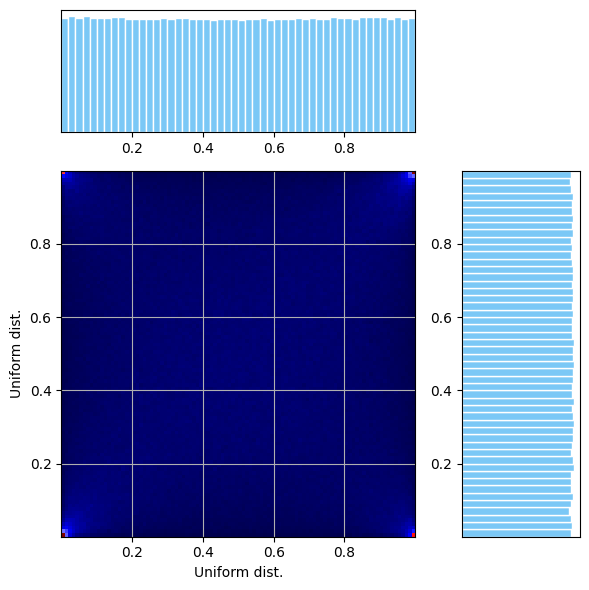
\includegraphics[width=0.45\textwidth]{figures/t-copula_2d}
\quad
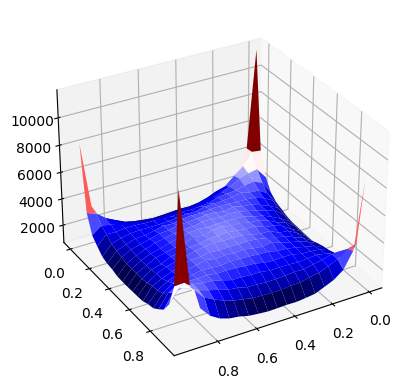
\includegraphics[width=0.5\textwidth]{figures/t-copula_3d}
\caption{Graphical representations of the t-copula, 2D on the left, 3D on the right.}
\label{fig:t-copula}
\end{figure}

\subsection{Copula Types}
There are numerous types of copula but two are the main classes: one-factor and two-factor copulas.
The most popular one-factor copulas are the Gaussian and the Archimedean. The latter can be split further into Gumbel, Clayton, and Frank copulas.
Two-factor copulas include the student’s t, Frechet, and Marshal-Olkin copula. 
We are going to concentrate on the Gaussian copula only though.

\section{One Factor Gaussian Copula Model}
While there are several types of copula function models, the first introduced was the \emph{one-factor Gaussian copula model}. This model is quite simple and has, above all, the advantage that can be solved analytically. 

In essence the one-factor Gaussian copula, is nothing but a numerical algorithm to generate samples of normally distributed random variables that have a given (Gaussian) pair-wise correlation. 

Consider a portfolio of $N$ bonds and assume that the marginal default probabilities are known for each issuer. Define:

\begin{itemize}
\tightlist
\item
$t_i$, the time of default of the $i^{th}$ company:
\item $Q_i(t)$, the cumulative probability that company $i$ will default before time $t$; that is, the probability that $t_i \le t$.
\end{itemize}

To generate a one-factor model for the default times ($t_i$) we define random variables $X_i$ $(1\le i \le N)$
\begin{equation}
X_i = a_i M + \sqrt{1-a_i^2}Z_i,\qquad i = 1, 2,\ldots, N
\label{eq:normalized_var}
\end{equation}
where $M$ and the $Z_i$ are independent zero-mean unit-variance  distributions (hence $X_i$ are also distributed with zero-mean and unit standard-deviation) and $-1 \le a_i < 1$.

Eq.~\ref{eq:normalized_var} defines a correlation structure between the $X_i$ which are dependent on a single common factor $M$. The $Z_i$ term is called the \emph{idiosyncratic component} of default. The particular functional form of Eq.~\ref{eq:normalized_var} has been chosen to ensure the desired correlation structure among the $X_i$. Indeed the correlation between $X_i$ and $X_j$ is

\begin{equation*}
\rho(X_i, X_j) = \cfrac{\mathbb{E}[(X_i-\mu_i)(X_j-\mu_j)]}{\sigma_{i}\sigma_{j}} = \mathbb{E}[X_i X_j] = a_i a_j \mathbb{E}[M^2] = a_i a_j
\end{equation*}
where we just exploit the definition of $X_i$ and its properties.

%Assume that the $i^{th}$ company has defaulted by the time $t_i$ if $X_i$ is below a threshold value $\bar{x}_i(t_i)$.
If $F_i$ is the cumulative distribution function of $X_i$, with an inverse transform (see Section~\ref{distribution-transformation}) we can map $X_i$ to $t_i$, so that $Q_i(t_i) = P(X_i\le x)=F_i(x)$. Therefore a point $X_i = x$ is transformed to $t_i = t$ with $x = F_i^{-1}[Q_i(t)]$ connecting the marginal distribution of the copula model to the default times.

Let's note that, \textbf{conditional} on $M$, the $N$ default events are \textbf{independent}. So we can write
\begin{equation}
\begin{split}
Q_i^{\textrm{corr}}(t_i|M) = P(X_i\le x|M) &= P(a_i M + \sqrt{1-a_i^2}Z_i\le x) =\\
&= P\left(Z_i\le \cfrac{x-a_i M}{\sqrt{1-a_i^2}}\right)
=H_i\left(\cfrac{F^{-1}[Q(t_i)]-a_i M}{\sqrt{1-a_i^2}}\right)
\end{split}
\label{eq:generic_copula}
\end{equation}
where $H_i$ is the cumulative distribution function of the $Z_i$.

Although in principle any distribution could be used for $M$ and the $Z$'s (provided they have zero mean and unit variance), one common choice is to let them be standard normal distributions (resulting in a Gaussian copula).
So we can rewrite Eq.~\ref{eq:generic_copula} as

\begin{equation}
Q_i^{\textrm{corr}}(t_i|M) = \Phi\left(\cfrac{\Phi^{-1}[Q(t_i)]-a_i M}{\sqrt{1-a_i^2}}\right)
\label{eq:gaussian_one_factor_copula}
\end{equation}
where $\Phi$ denotes the standard normal cumulative distribution function.

If we call $\mathcal{C}(t_1,\ldots,t_N)$ the joint distribution of the default times of the $N$ bonds in the portfolio then

\begin{equation}
\mathcal{C}(t_1,\ldots,t_N, \rho)=\Phi_{N}(\Phi^{-1}(Q_1(t_1)),\ldots,\Phi^{-1}(Q_N(t_N)), \boldsymbol{\rho})
\label{eq:gaussian_copula}
\end{equation}
where $\boldsymbol{\rho}$ represents the correlation matrix of the default probabilities. Eq.~\ref{eq:gaussian_copula} is the one factor Gaussian copula model (one factor because there is only a random variable, $M$, which determines the correlation between $X_i$).

Different distribution choices result in different copula models, and in various natures of the default dependence. For example, copulas where the $M$ have heavy tails, generate models where there is a greater likelihood of a early defaults clustering for several companies.

\subsubsection{Standard Market Model}
\label{standard-market-model}

Consider the following two assumptions:

\begin{itemize}
\tightlist
\item all the companies have the same default intensity (hazard rates), i.e, $\lambda_i = \lambda$ (which means they all have the same default probabilities $Q_i = Q$);
\item the pairwise default correlations are the same, i.e $a_i = a$; in other words the contribution of the market component $M$ is the same for all the companies and the correlation between any two companies is constant, $\rho = a^2$.
\end{itemize}

Given the market situation $M = m$, all companies have the same cumulative default probability $Q_i^{\textrm{corr}}(t_i|m)=P(X_i < x|m)$. 

In this case the one factor Gaussian model is also called \emph{Market Standard Model}. Later in this Notes we will also see how the correlation used in Eq.~\ref{eq:gaussian_one_factor_copula} can be implied from the market quotes of credit derivatives.

Letting $l(t|m)$ be the total defaults that have occurred by time $t$ conditional on the market condition $M = m$, then $l(t|m)$ follows a binomial distribution (see Appendix~\ref{binomial-distribution}), and the probability of default of $j$ companies can be expressed as

\begin{equation}
P_{\mathrm{def}}(l(t|m) = j) = \cfrac{N!}{j!(N-j)!}(Q_i^{\textrm{corr}}(t_i|m))^j(1-Q_i^{\textrm{corr}}(t_i|m))^{N-j},\qquad  j=0, 1, 2,\ldots,N
\end{equation}

In general to evaluate any function $g(P_{\mathrm{def}}[l(t)])$ regardless the value of one its factor ($M$) (e.g. an NPV or a fair value), is necessary to average according to all possible values that this factor can take. The average is performed by integrating over the market factor (i.e. this is equivalent to perform a weighted sum of $g$ with the probability distribution of the factor).  

\begin{equation}
g(P_{\mathrm{def}}(l(t) = j)) = \int_{-\infty}^{\infty}{g(P_{\mathrm{def}}[l(t|m) = j])\cdot f_M(m)dm}
\label{eq:gaussian_quadrature}
\end{equation}

In the general case where the default probabilities of each company are not the same it is possible to determine $P_{\mathrm{def}}[l(t|M)=j]$ through an iterative procedure before proceeding with the integration of Eq.~\ref{eq:gaussian_quadrature}. An example of this iterative technique will be shown in Section~\ref{sec:expected_losses}.

\subsection{Extensions of the One Factor Copula Model}
Many other one-factor model have been studied: t-Student copula, Clayton copula,\ldots In general we can define a new model by simply choosing particular functional forms for $M$ and $Z_i$ in Eq.~\ref{eq:normalized_var} provided they are with zero mean and standard deviation one. 

If instead of the single factor $M$ there are two or more, Eq.~\ref{eq:normalized_var} becomes

\begin{equation}
X_i = a_1 M_1 + a_2 M_2 + \sqrt{1 - a_1^2 - a^2_2}Z_i
\end{equation}
and similarly
\begin{equation}
Q^{\textrm{corr}}(t|M_1, M_2) = \Phi\left(\cfrac{\Phi^{-1}[Q(t)]-a_1 M_1 - a_2 M_2}{\sqrt{1 - a_1^2 - a^2_2}}\right)
\end{equation}
In terms of computation time, this kind of models are proportionally slower with the increase of the factor numbers, since the integration of Eq.~\ref{eq:gaussian_quadrature} has to be carried on each factor of the model.

\section{Complex Correlation Structures and the Financial Crisis}
\label{complex-correlation-structures-and-the-financial-crisis}

In the derivation of the Gaussian Copula Model we have used the normal distribution. However, we could have used other and more complex copulas as well. For example we might want to assume the correlation is non-symmetric which is useful in finance when correlations become very strong during market crashes and returns very negative.

In fact, Gaussian copulas are said to have played a key role in the 2008 financial crisis as tail-correlations were severely underestimated. Consider a set of mortgages in a CDO (a kind of derivative that will be described in the next Chapter): they are clearly correlated, since if one mortgage fails, the likelihood that another failing is increased. In the early 2000s, the banks only knew how to model the marginals of the default rates. Then an (in)famous paper by Li~\cite{bib:copula_li} suggested to use Gaussian copulas to model the correlations between those marginals. Rating agencies relied on this model so heavily, that severely underestimated the risk and gave false ratings\ldots

If you are interested in the argument read this paper~\cite{bib:copula_and_2008} for an excellent description of Gaussian copulas and the Financial Crisis, which argues that different copula choices would not have made a difference but instead the assumed correlation was way too low.

\section*{Exercises}
\begin{question}
Using the \emph{probability integral transform} transform a Gumbel distribution into a Gaussian. Plot also all the distributions involved in the transformation.
\end{question}

\cprotEnv\begin{solution}
\begin{ipython}
from scipy.stats import gumbel_l, norm
from matplotlib import pyplot as plt

gumbel = gumbel_l()
xg = gumbel.rvs(100000)
xu = gumbel.cdf(xg)
xn = norm.ppf(xu)

sub1 = plt.subplot(1, 3, 1)
sub1.hist(xg, 50)
sub1.grid(True)
sub1.set_xlabel("$x_{gumbel}$")
sub2 = plt.subplot(1, 3, 2)
sub2.hist(xu, 50)
sub2.grid(True)
sub2.set_xlabel("$x_{uniform}$")
sub3 = plt.subplot(1, 3, 3)
sub3.hist(xn, 50)
sub3.grid(True)
sub3.set_xlabel("$x_{normal}$")
plt.show()
\end{ipython}

\begin{figure}[htbp]
\begin{center}
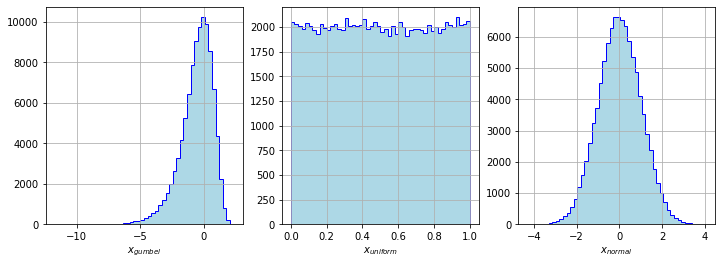
\includegraphics[width=0.9\linewidth]{figures/ex_gumbel_to_gauss.png}
\end{center}
\end{figure}
\end{solution}

\begin{question}
Without using the corresponding \texttt{rvs()} method try to generate 10 random numbers distributed as Beta distribution (parameters \texttt{a=3} and \texttt{b=10}).

\noindent\textbf{Hint:} starts with generating uniformly distributed random numbers.
\end{question}	

\cprotEnv\begin{solution}
\begin{ipython}
from scipy.stats import beta, uniform

x = uniform.rvs(size=10)
b = beta(a=3, b=10)
x_b = b.ppf(x)

print (x_b)
\end{ipython}
\begin{ioutput}
[0.29190237 0.45669406 0.10336582 0.5403107 0.08305872 0.32425694
0.43902811 0.11820592 0.28659784 0.22316621]
\end{ioutput}
\end{solution}

\begin{question}
Consider two companies whose default probabilities as a function of time are modeled according to a lognormal distribution with $\sigma =0.5$ (\texttt{scipy.stats.lognorm(0.5)}). Compare the joint 2D distributions in case of no correlation and with a Gaussian correlation of 0.8.

\noindent\textbf{Hint:} to plot the joint distribution use \texttt{matplotlib} function \texttt{hist2d(x1, x2, range=[[x1min, x1max], [xmin, x2max]], bins=(50, 50)) }.
\end{question}

\cprotEnv\begin{solution}
\begin{ipython}
from scipy.stats import lognorm, multivariate_normal, norm
import numpy

numpy.random.seed(1)
samples = 1000000
l1_uncorr = lognorm(0.5).rvs(size=samples)
l2_uncorr = lognorm(0.5).rvs(size=samples)
mvnorm = multivariate_normal(mean = (0, 0), 
                             cov = [[1, 0.8],
                                    [0.8, 1]])
x = mvnorm.rvs(size=samples)
x_corr = norm.cdf(x)
l1_corr = lognorm(0.5).ppf(x_corr[:, 0])
l2_corr = lognorm(0.5).ppf(
x_corr[:, 1])
plt.figure(figsize=(12, 4))
sub1 = plt.subplot(1, 2, 1)
sub1.hist2d(l1_uncorr, l2_uncorr, range=[[0, 2], [0, 2]], bins=(100, 100))
sub2 = plt.subplot(1, 2, 2)
sub2.hist2d(l1_corr, l2_corr, range=[[0, 2], [0, 2]], bins=(100, 100))
plt.show()
\end{ipython}
\noindent 
The resulting comparison is shown in Fig.~\ref{fig:joint_2d}.
\begin{figure}[htbp]
\begin{center}
	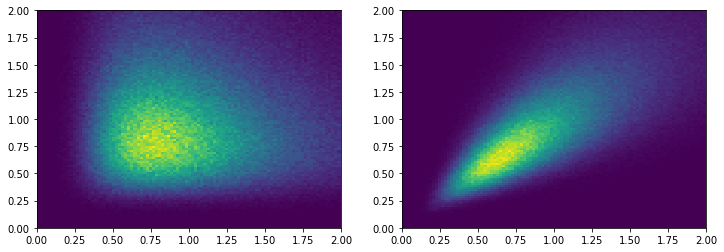
\includegraphics[width=0.9\linewidth]{figures/copula_lognormal.png}
\end{center}
\caption{Comparision of the joint 2D distributions in case of no correlation (left) and with a Gaussian correlation of 0.8 (right).}
\label{fig:joint_2d}
\end{figure}

In order to quantify the difference shown with the comparison of the two 2D plots we can calculate the probability that both companies default in the next six months.

So the probability that a single company default in six months regardless the other can be calculated from the \texttt{cdf} of the lognormal distribution.
Hence in case of independent probabilities what required is just the squared of this value (about 0.07\%).

\begin{ipython}
default_6m = lognorm(0.5).cdf(.5)
print(default_6m**2)
\end{ipython}
\begin{ioutput}
0.006860563560014724
\end{ioutput}

In the case of correlation instead we have to loop over the samples from the joint multivariate distribution (with correlation) and check how many times both values are less than \texttt{default\_6m}.

\begin{ipython}
success = 0.0
for i in range(samples):
    if max(x_corr[i]) < default_2:
        success += 1

print (success/samples)
\end{ipython}
\begin{ioutput}
0.044654
\end{ioutput}

This result can be interpreted graphically by saying that the entries in the "square" $[0, 0.5]$ in the left histogram are about 0.7\% of the total while the entries in the right plot in same "square" are about 4.5\% of the total. 
\end{solution}


